% This is samplepaper.tex, a sample chapter demonstrating the
% LLNCS macro package for Springer Computer Science proceedings;
% Version 2.20 of 2017/10/04
%
%\documentclass[runningheads]{report}
\documentclass{article}
%
\usepackage{graphicx}
\usepackage{comment}
\usepackage{indentfirst}
\usepackage{float}
% Used for displaying a sample figure. If possible, figure files should
% be included in EPS format.
%
% If you use the hyperref package, please uncomment the following line
% to display URLs in blue roman font according to Springer's eBook style:
% \renewcommand\UrlFont{\color{blue}\rmfamily}

\begin{document}
%
\title{ECE219 Project 3\\ Collaborative Filtering}
%
%\titlerunning{Abbreviated paper title}
% If the paper title is too long for the running head, you can set
% an abbreviated paper title here
%
\author{Zhilai~Shen, Yufei~Hu, Zheang~Huai, and Tianyi~Liu \\
105023454, 404944367, 505222324, 705035425
}
%
% First names are abbreviated in the running head.
% If there are more than two authors, 'et al.' is used.
%              % typeset the header of the contribution

%
%
%
%
\begin{comment}
\section{First Section}
\subsection{A Subsection Sample}
Please note that the first paragraph of a section or subsection is
not indented. The first paragraph that follows a table, figure,
equation etc. does not need an indent, either.

Subsequent paragraphs, however, are indented.

\subsubsection{Sample Heading (Third Level)} Only two levels of
headings should be numbered. Lower level headings remain unnumbered;
they are formatted as run-in headings.

\paragraph{Sample Heading (Fourth Level)}
The contribution should contain no more than four levels of
headings. Table~\ref{tab1} gives a summary of all heading levels.

\begin{table}
\caption{Table captions should be placed above the
tables.}\label{tab1}
\begin{tabular}{|l|l|l|}
\hline
Heading level &  Example & Font size and style\\
\hline
Title (centered) &  {\Large\bfseries Lecture Notes} & 14 point, bold\\
1st-level heading &  {\large\bfseries 1 Introduction} & 12 point, bold\\
2nd-level heading & {\bfseries 2.1 Printing Area} & 10 point, bold\\
3rd-level heading & {\bfseries Run-in Heading in Bold.} Text follows & 10 point, bold\\
4th-level heading & {\itshape Lowest Level Heading.} Text follows & 10 point, italic\\
\hline
\end{tabular}
\end{table}


\noindent Displayed equations are centered and set on a separate
line.
\begin{equation}
x + y = z
\end{equation}
Please try to avoid rasterized images for line-art diagrams and
schemas. Whenever possible, use vector graphics instead (see
Fig.~\ref{fig1}).

\begin{figure}[!htbp]
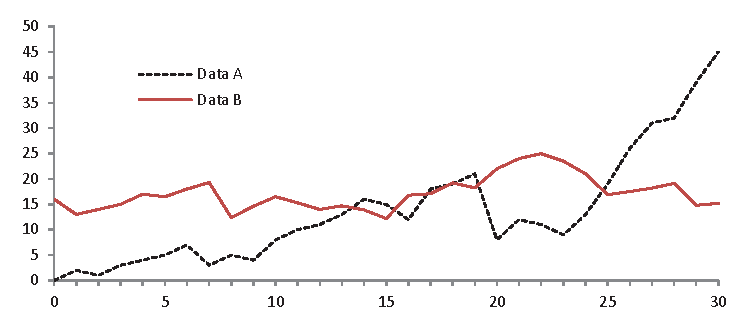
\includegraphics[width=\textwidth]{Figure/fig1.eps}
\caption{A figure caption is always placed below the illustration.
Please note that short captions are centered, while long ones are
justified by the macro package automatically.} \label{fig1}
\end{figure}

\begin{theorem}
This is a sample theorem. The run-in heading is set in bold, while
the following text appears in italics. Definitions, lemmas,
propositions, and corollaries are styled the same way.
\end{theorem}
%
% the environments 'definition', 'lemma', 'proposition', 'corollary',
% 'remark', and 'example' are defined in the LLNCS documentclass as well.
%
\begin{proof}
Proofs, examples, and remarks have the initial word in italics,
while the following text appears in normal font.
\end{proof}
For citations of references, we prefer the use of square brackets
and consecutive numbers. Citations using labels or the author/year
convention are also acceptable. The following bibliography provides
a sample reference list with entries for journal
articles~\cite{ref_article1}, an LNCS chapter~\cite{ref_lncs1}, a
book~\cite{ref_book1}, proceedings without editors~\cite{ref_proc1},
and a homepage~\cite{ref_url1}. Multiple citations are grouped
\cite{ref_article1,ref_lncs1,ref_book1},
\cite{ref_article1,ref_book1,ref_proc1,ref_url1}.
%
% ---- Bibliography ----
%
% BibTeX users should specify bibliography style 'splncs04'.
% References will then be sorted and formatted in the correct style.
%
% \bibliographystyle{splncs04}
% \bibliography{mybibliography}
%

\end{comment}

\begin{titlepage}
	\centering
	\includegraphics[width=0.15\textwidth]{UCLA.png}\par\vspace{1cm}
	\vspace{1cm}
	{\scshape\Large ECE219 Project 5 \par}
	\vspace{1.5cm}
	{\huge\bfseries Application - Twitter data\par}
	\vspace{2cm}
	{\Large\itshape Zhilai~Shen, Yufei~Hu, Zheang~Huai, and Tianyi~Liu\par}
	{\Large\itshape 105023454, 404944367, 505222324, 705035425\par}
	\vfill

	\vfill

% Bottom of the page
	{\large \today\par}
\end{titlepage}

\tableofcontents

\newpage

\section{Popularity Prediction}
\subsection{A first look at the data}
\textbf{Question 1:}

The statistics for each hashtag are as follows.\\

Statistics for \#GoHawks

Average number of tweets per hour: $292.488$

Average number of followers of users posting the tweets per tweet: $2217.924$

Average number of retweets per tweet: $2.0132$\\

Statistics for \#GoPatriots

Average number of tweets per hour: $40.955$

Average number of followers of users posting the tweets per tweet: $1427.253$

Average number of retweets per tweet: $1.408$\\

Statistics for \#NFL

Average number of tweets per hour: $397.021$

Average number of followers of users posting the tweets per tweet: $4662.375$

Average number of retweets per tweet: $1.534$\\

Statistics for \#Patriots

Average number of tweets per hour: $750.894$

Average number of followers of users posting the tweets per tweet: $3280.464$

Average number of retweets per tweet: $1.785$\\

Statistics for \#SB49

Average number of tweets per hour: $1276.857$

Average number of followers of users posting the tweets per tweet: $10374.160$

Average number of retweets per tweet: $2.527$\\

Statistics for \#SuperBowl

Average number of tweets per hour: $2072.118$

Average number of followers of users posting the tweets per tweet: $8814.968$

Average number of retweets per tweet: $2.391$\\



\bigbreak
\textbf{Question 2:}

\begin{figure}
\centering
\scalebox{0.6}{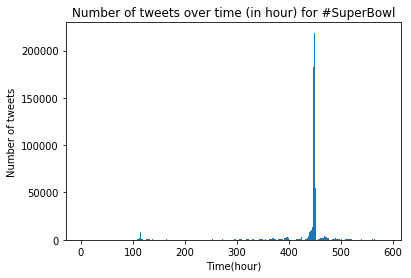
\includegraphics{Figure/Q2_1.png}}
\caption{Number of tweets over time for \#SuperBowl} \label{Q2_1}
\end{figure}

\begin{figure}
\centering
\scalebox{0.6}{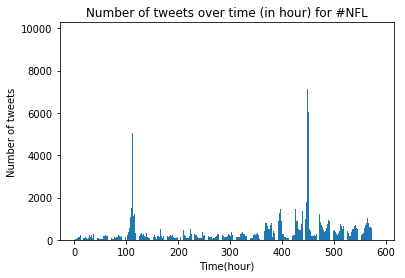
\includegraphics{Figure/Q2_2.png}}
\caption{Number of tweets over time for \#NFL} \label{Q2_2}
\end{figure}

The plots of number of tweets in hour over time for \#SuperBowl and \#NFL can be seen in Figure \ref{Q2_1},Figure \ref{Q2_2}.


\bigbreak
\subsection{Linear regression}
\textbf{Question 3:}

\begin{table}[h]
\center
\caption{MSE and R-squared measure}
\scalebox{0.9}{
\begin{tabular}{c|c|c}
\hline
hashtag & MSE & R-squared measure \\\hline
\#GoHawks & $758554.248$ & $0.504$ \\\hline
\#GoPatriots & $27583.582$ & $0.637$ \\\hline
\#NFL & $269962.153$ & $0.652$ \\\hline
\#Patriots & $5180890.103$ & $0.679$ \\\hline
\#SB49 & $16180394.455$ & $0.808$ \\\hline
\#SuperBowl & $52483472.229$ & $0.803$ \\\hline
\end{tabular}}
\label{Q3_11}
\end{table}


The models' Mean Squared Error(MSE) and R-squared measure for each hashtag can be seen in Table \ref{Q3_11}. The results of t-test and p-values can be seen in Figure \ref{Q3_1}, \ref{Q3_2}, \ref{Q3_3}, \ref{Q3_4}, \ref{Q3_5}, \ref{Q3_6}. x1-x5 represents Number of tweets, Total number of retweets, Sum of the number of followers of the users, Maximum number of followers of the users, Time of the day, respectively.

From p-values, we can get the significance of each feature for every hashtag, i.e., The feature with smaller p-value has higher significance. In general, number of tweets has low p-value for every hashtag and therefore it's a very significant feature.

\textbf{Note: Here I follow the same instruction as in Question1 "if a users posted twice, we count the user and the user’s followers twice as well", when I calculate sum of the number of followers of the users.}

\begin{figure}
\centering
\scalebox{0.6}{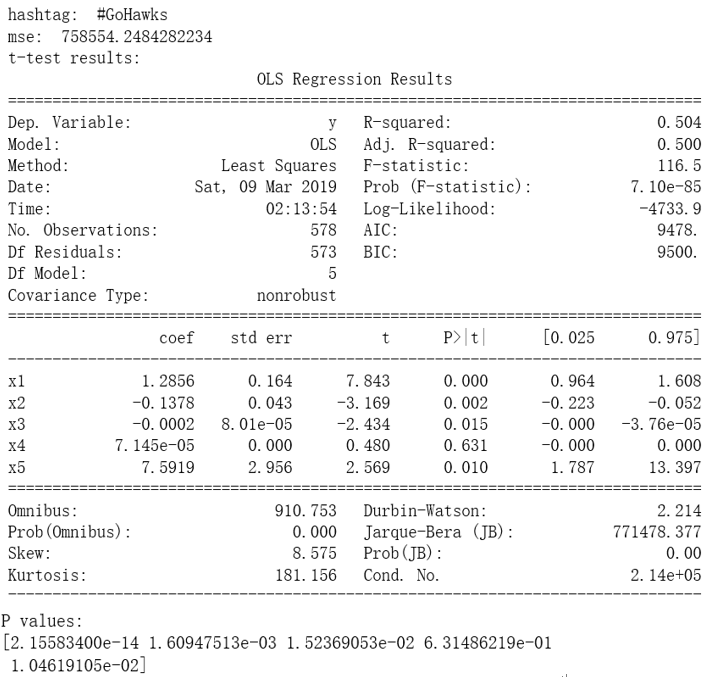
\includegraphics{Figure/Q3_1.png}}
\caption{t-test and p-values for \#GoHawks} \label{Q3_1}
\end{figure}

\begin{figure}
\centering
\scalebox{0.6}{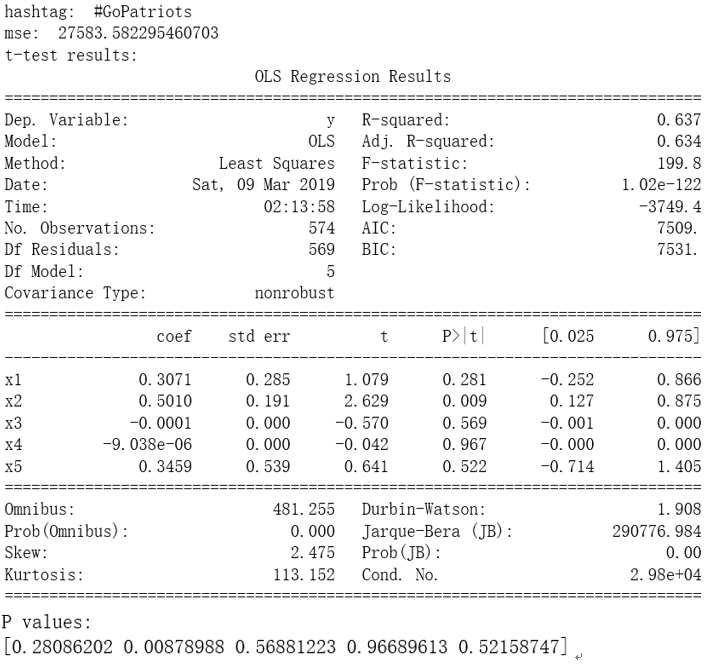
\includegraphics{Figure/Q3_2.png}}
\caption{t-test and p-values for \#GoPatriots} \label{Q3_2}
\end{figure}

\begin{figure}
\centering
\scalebox{0.6}{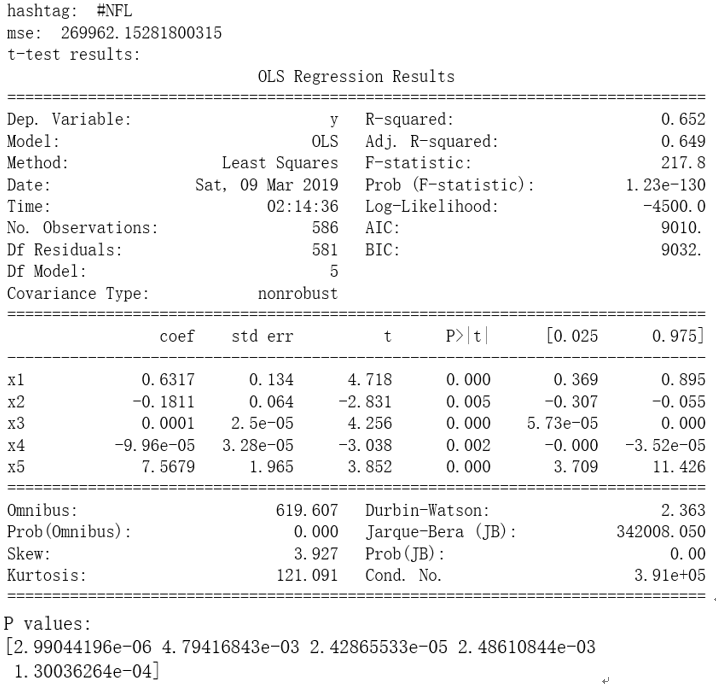
\includegraphics{Figure/Q3_3.png}}
\caption{t-test and p-values for \#NFL} \label{Q3_3}
\end{figure}

\begin{figure}
\centering
\scalebox{0.6}{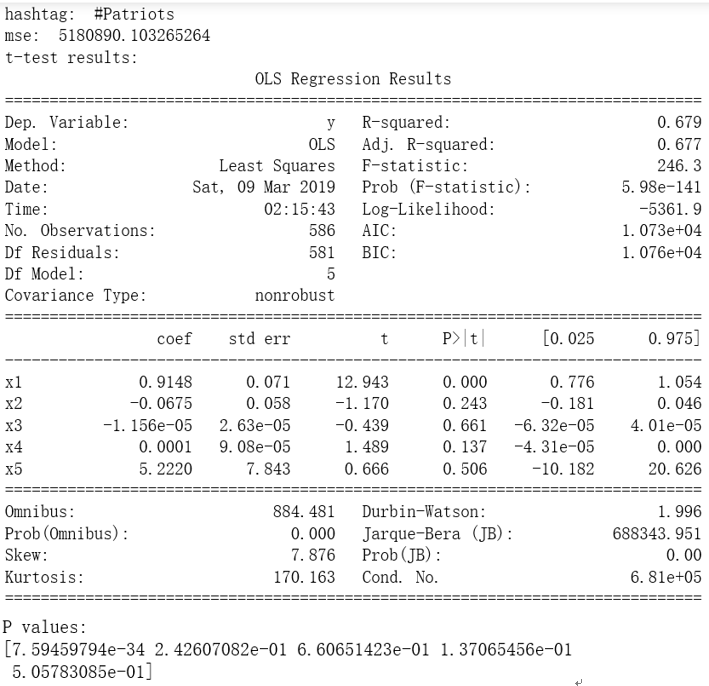
\includegraphics{Figure/Q3_4.png}}
\caption{t-test and p-values for \#Patriots} \label{Q3_4}
\end{figure}

\begin{figure}
\centering
\scalebox{0.6}{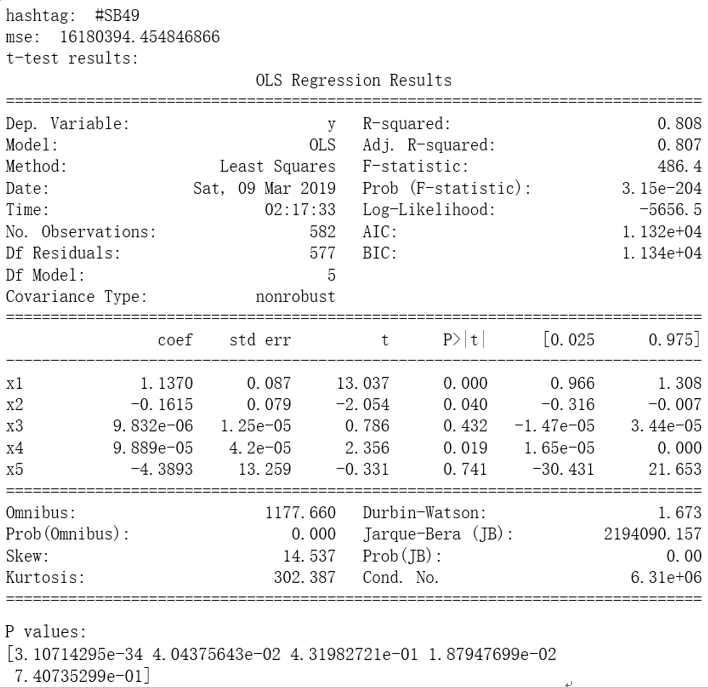
\includegraphics{Figure/Q3_5.png}}
\caption{t-test and p-values for \#SB49} \label{Q3_5}
\end{figure}

\begin{figure}
\centering
\scalebox{0.6}{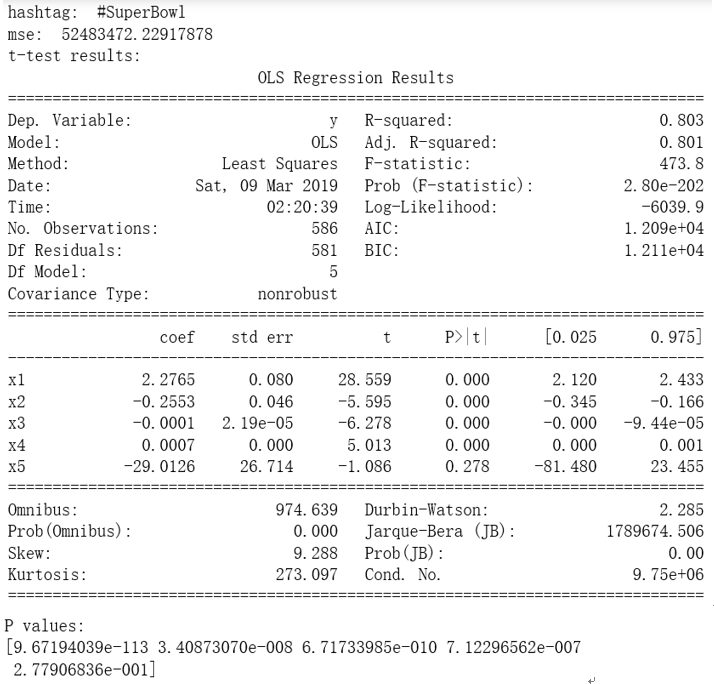
\includegraphics{Figure/Q3_6.png}}
\caption{t-test and p-values for \#SuperBowl} \label{Q3_6}
\end{figure}


\bigbreak
\subsection{Feature analysis}
\textbf{Question 4:}

The new features we find useful for this problem are:

-Url ratio. A url in Twitter can be a link of a picture, a song, a video, or a piece of news. High ratio of tweets with urls may indicate a topic about a good song, an interesting picture or video, or a piece of breaking news. In our project, we used “url count” to represent “url ratio”.

-Author count. Besides tweet count for a hashtag, we also consider the unique number of authors who posted tweets containing the hashtag. This feature can be used to recognize those hashtags automatically posted by some fake accounts.

-Mention count. Mention is a directional sharing behavior in Twitter. Messages can be shared to a designated user using @ as the prefix of the user’s name. If a user was mentioned in a tweet with a hashtag, he probably took part in the topic, especially when this mention came from his friends.

-Ranking score. Ranking scores are listed in each tweet to show its scores intuitively, which
shows its spread ability.

-Number of hashtags. Sometimes, some hashtags are not used individually, but are used together with other hashtags, e.g. \#boston\#explosion. It's reasonable to guess the number of hashtag in tweets are critical to indicate the popularity of the topic.
\\

\begin{table}[h]
\center
\caption{MSE and R-squared measure(after adding new features)}
\scalebox{0.9}{
\begin{tabular}{c|c|c}
\hline
hashtag & MSE & R-squared measure \\\hline
\#GoHawks & $485098.424$ & $0.684$ \\\hline
\#GoPatriots & $8182.927$ & $0.892$ \\\hline
\#NFL & $163901.087$ & $0.791$ \\\hline
\#Patriots & $2922872.021$ & $0.819$ \\\hline
\#SB49 & $12387685.9921$ & $0.853$ \\\hline
\#SuperBowl & $30825995.718$ & $0.884$ \\\hline
\end{tabular}}
\label{Q4_11}
\end{table}


After adding these five new features, the models' Mean Squared Error(MSE) and R-squared measure for each hashtag can be seen in Table \ref{Q4_11}. The results of t-test and p-values can be seen in Figure \ref{Q4_1}, \ref{Q4_2}, \ref{Q4_3}, \ref{Q4_4}, \ref{Q4_5}, \ref{Q4_6}. x1-x10 represents Number of tweets, Total number of retweets, Sum of the number of followers of the users, Maximum number of followers of the users, Time of the day, Url number, Author count, Mention count, Ranking score, Number of hashtags, respectively. From p-values, we can get the significance of each feature for every hashtag, i.e., The feature with smaller p-value has higher significance.

\begin{figure}
\centering
\scalebox{0.6}{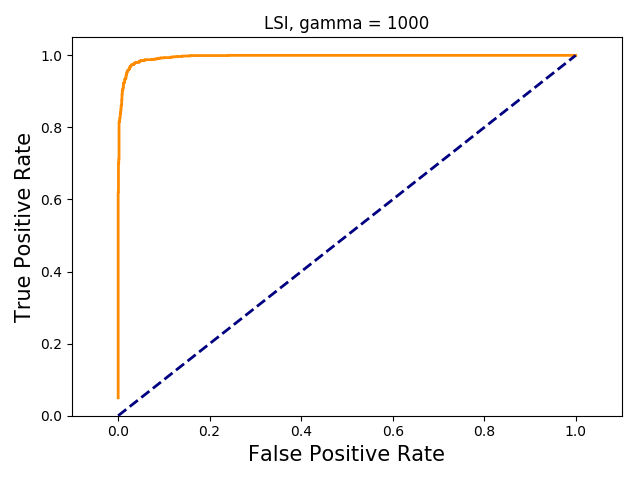
\includegraphics{Figure/Q4_1.png}}
\caption{t-test and p-values for \#GoHawks(after adding new features)} \label{Q4_1}
\end{figure}

\begin{figure}
\centering
\scalebox{0.6}{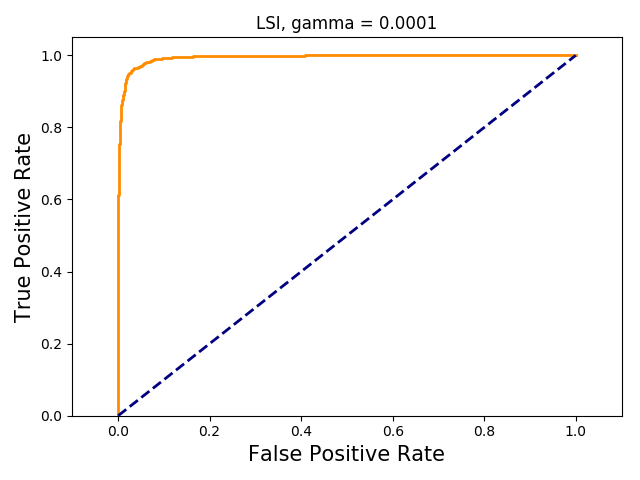
\includegraphics{Figure/Q4_2.png}}
\caption{t-test and p-values for \#GoPatriots(after adding new features)} \label{Q4_2}
\end{figure}

\begin{figure}
\centering
\scalebox{0.6}{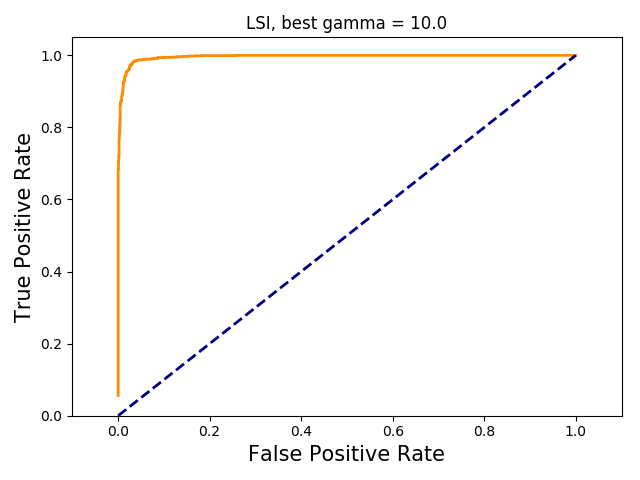
\includegraphics{Figure/Q4_3.png}}
\caption{t-test and p-values for \#NFL(after adding new features)} \label{Q4_3}
\end{figure}

\begin{figure}
\centering
\scalebox{0.6}{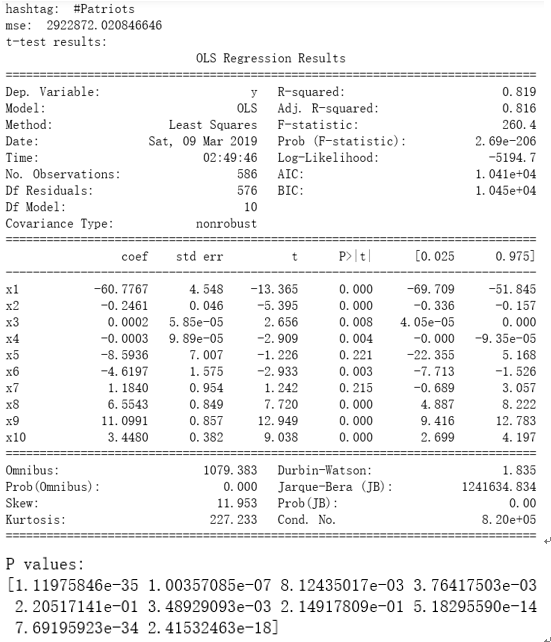
\includegraphics{Figure/Q4_4.png}}
\caption{t-test and p-values for \#Patriots(after adding new features)} \label{Q4_4}
\end{figure}

\begin{figure}
\centering
\scalebox{0.6}{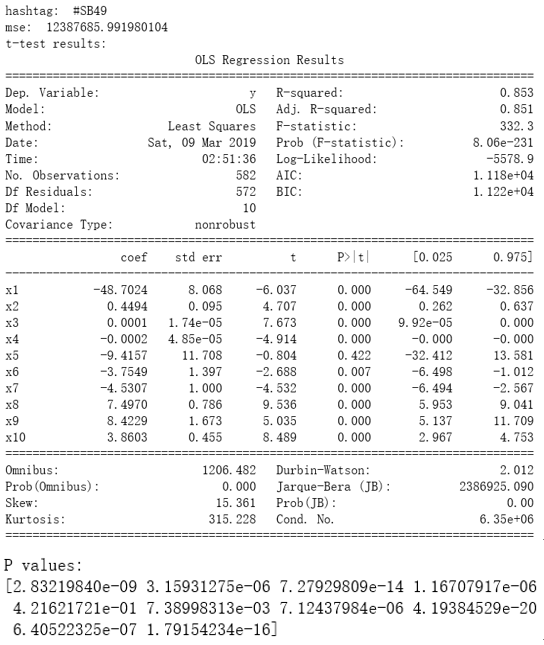
\includegraphics{Figure/Q4_5.png}}
\caption{t-test and p-values for \#SB49(after adding new features)} \label{Q4_5}
\end{figure}

\begin{figure}
\centering
\scalebox{0.6}{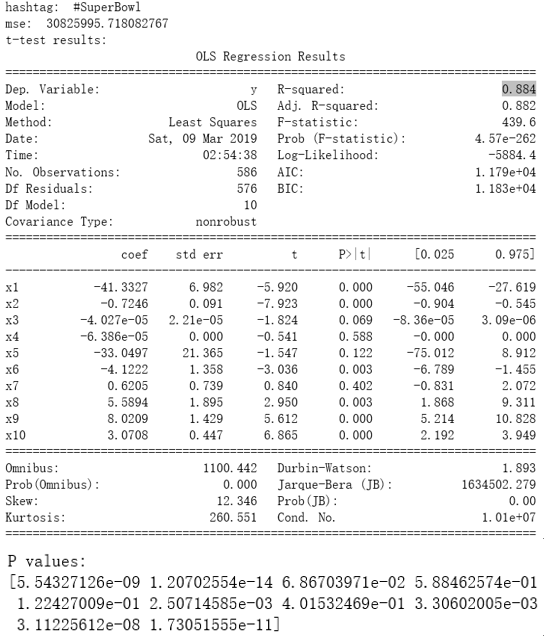
\includegraphics{Figure/Q4_6.png}}
\caption{t-test and p-values for \#SuperBowl(after adding new features)} \label{Q4_6}
\end{figure}



\bigbreak
\textbf{Question 5:}

\begin{figure}
\centering
\scalebox{0.6}{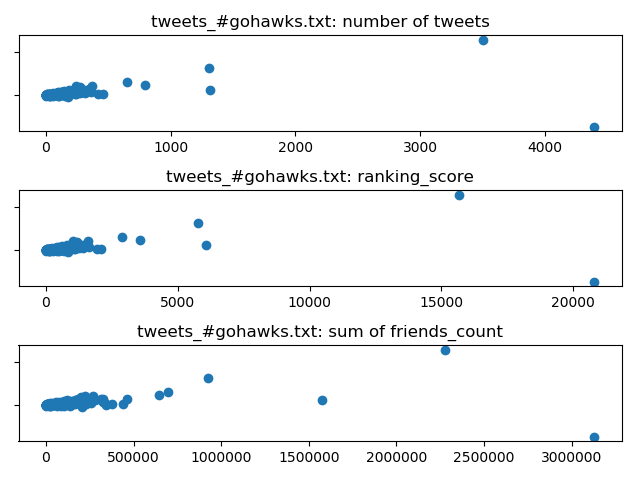
\includegraphics{Figure/Q5_1.png}}
\caption{Predictant versus value of that feature (tweets\_\#gohawks)} \label{Q5_1}
\end{figure}

\begin{figure}
\centering
\scalebox{0.6}{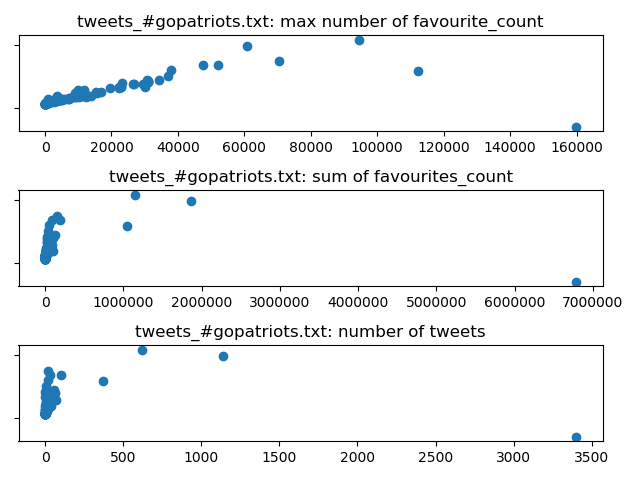
\includegraphics{Figure/Q5_2.png}}
\caption{Predictant versus value of that feature (tweets\_\#gopatriots.txt)} \label{Q5_2}
\end{figure}

\begin{figure}
\centering
\scalebox{0.6}{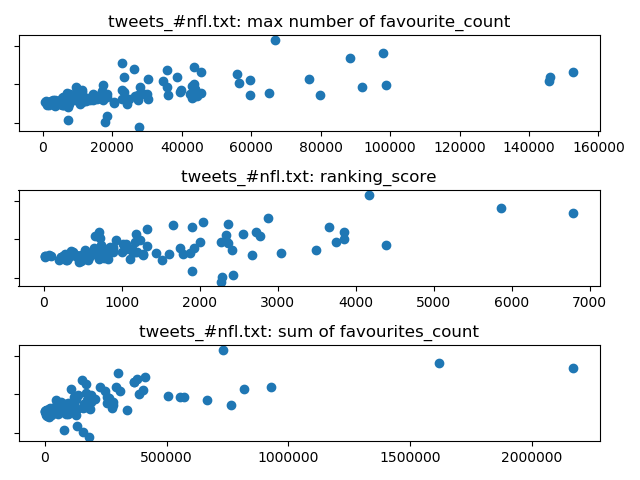
\includegraphics{Figure/Q5_3.png}}
\caption{Predictant versus value of that feature (tweets\_\#nfl.txt)} \label{Q5_3}
\end{figure}

\begin{figure}
\centering
\scalebox{0.6}{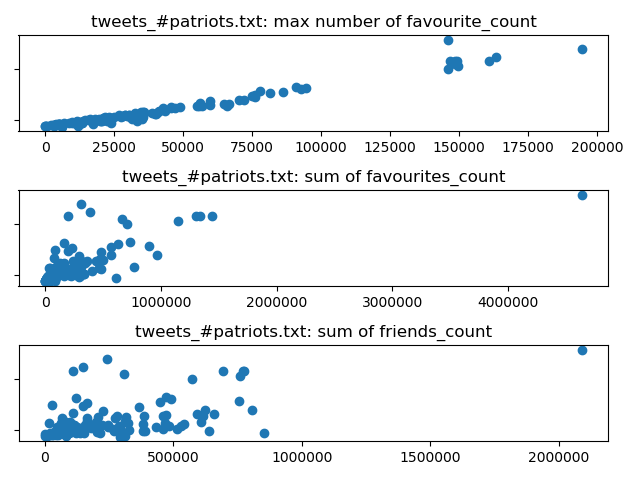
\includegraphics{Figure/Q5_4.png}}
\caption{Predictant versus value of that feature (tweets\_\#patriots.txt)} \label{Q5_4}
\end{figure}

\begin{figure}
\centering
\scalebox{0.6}{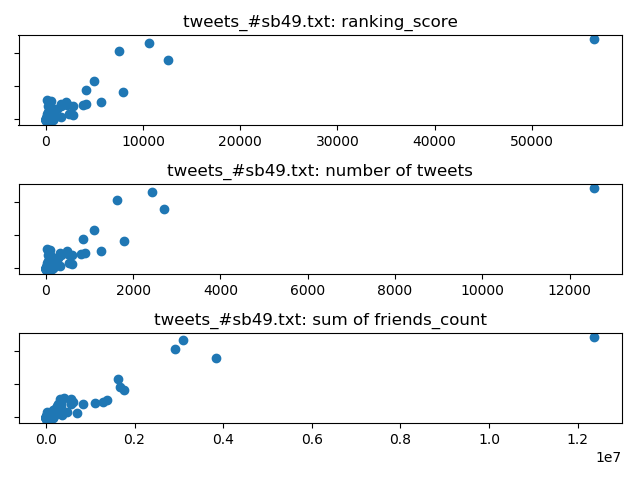
\includegraphics{Figure/Q5_5.png}}
\caption{Predictant versus value of that feature (tweets\_\#sb49.txt)} \label{Q5_5}
\end{figure}

\begin{figure}
\centering
\scalebox{0.6}{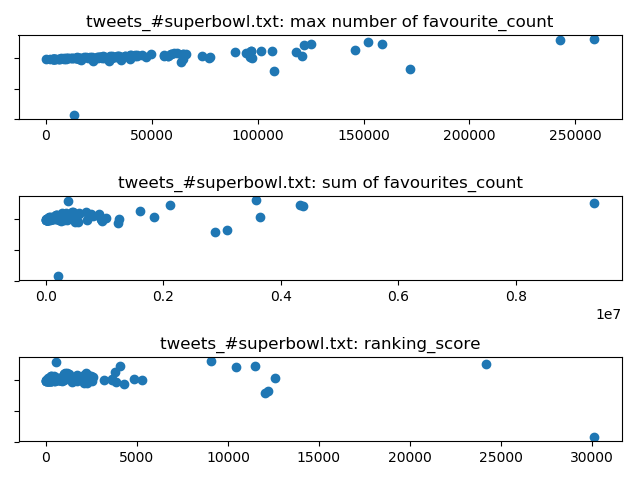
\includegraphics{Figure/Q5_6.png}}
\caption{Predictant versus value of that feature (tweets\_\#superbowl.txt)} \label{Q5_6}
\end{figure}

The features that we explored are "number of tweets", "sum of favorites count", "max number of favorite count", "ranking score" and "sum of friends count". P-values are printed for each feature. The three features with smallest p-values are chose and their scatter plots are plotted. They all exhibit a linear relationship with label. All the regression coefficients highly agree with the trends in the plots.\newline

\indent For hashtag of tweets\_\#gohawks, RMSE=$869.425$, p\_values=[$3.25025270e-26$, $6.92524349e-01$, $7.21598480e-01$, $3.90685740e-26$, $8.97754600e-02$]. The three most important features are: number of tweets, ranking\_score, sum of friends\_count. The scatter plot can be found at \ref{Q5_1}.\newline

\indent For hashtag of tweets\_\#gopatriots, RMSE=$331.184$, p\_values=[$6.71573022e-01$, $9.22773132e-03$, $9.01922321e-07$, $9.42369949e-01$, $8.95680420e-01$]. The three most important features are: max number of favourite\_count, sum of favourites\_count, number of tweets. The scatter plot can be found at \ref{Q5_2}.\newline

\indent For hashtag of tweets\_\#nfl, RMSE=$452.804$, p\_values=[$1.97628176e-04$, $8.38477484e-05$, $9.40719365e-09$, $5.34746493e-05$, $8.63316750e-01$]. The three most important features are: max number of favourite\_count, ranking\_score, sum of favourites\_count. The scatter plot can be found at \ref{Q5_3}.\newline

\indent For hashtag of tweets\_\#patriots, RMSE=$841.246$, p\_values=[$8.13914091e-02$, $7.91170792e-08$, $6.03920658e-10$, $1.21197912e-01$, $6.33201420e-02$]. The three most important features are: max number of favourite\_count, sum of favourites\_count, sum of friends\_count. The scatter plot can be found at \ref{Q5_4}.\newline

\indent For hashtag of tweets\_\#sb49, RMSE=$4561.116$, p\_values=[$6.29387464e-16$, $7.17424978e-01$, $5.46720292e-02$, $2.99497856e-16$, $4.33849037e-13$]. The three most important features are: ranking\_score, number of tweets, sum of friends\_count. The scatter plot can be found at \ref{Q5_5}.\newline

\indent For hashtag of tweets\_\#superbowl, RMSE=$17719.564$, p\_values=[$1.59756651e-03$, $5.55823802e-05$, $1.37347540e-07$, $1.50896890e-03$, $5.02659534e-01$]. The three most important features are: max number of favourite\_count, sum of favourites\_count, ranking\_score. The scatter plot can be found at \ref{Q5_6}.\newline

\indent Based on the observations above, it is found that for different hashtags, we obtain different important features. But in general, "sum of favorites count", "max number of favorite count", and "sum of friends count" are the three most important attributes for prediction. Obviously, if a tweet is liked by a lot of people, it will retweet more compared with other tweets. Also, if a user has many friends in tweet, it will increase the probability of retweet. Number of tweets per hour and ranking score seems less important in these procedures.


\bigbreak
\subsection{Piece-wise linear regression}
\textbf{Question 6:}

\begin{table}[h]
\center
\caption{MSE and R2 Score for tweets\_\#gohawks}
\scalebox{0.9}{
\begin{tabular}{|c|c|c|c|}
\hline
& Before 02/01/8:00 & 02/01/8:00 to 8:00 PM & After 02/01/8:00 PM \\\hline
MSE & 3778766.452 & 296932.872 & 36309.293 \\\hline
R2 Score & -356.419 & -3.276 & 0.215 \\\hline
\end{tabular}}
\label{tab:Q6_1}
\end{table}

\begin{table}[h]
\center
\caption{MSE and R2 Score for tweets\_\#gopatriots}
\scalebox{0.9}{
\begin{tabular}{|c|c|c|c|}
\hline
& Before 02/01/8:00 & 02/01/8:00 to 8:00 PM & After 02/01/8:00 PM \\\hline
MSE & 5026.292 & 27119.285 & 217.526 \\\hline
R2 Score & -0.645 & -1.811 & -0.327 \\\hline
\end{tabular}}
\label{tab:Q6_2}
\end{table}

\begin{table}[h]
\center
\caption{MSE and R2 Score for tweets\_\#nfl}
\scalebox{0.9}{
\begin{tabular}{|c|c|c|c|}
\hline
& Before 02/01/8:00 & 02/01/8:00 to 8:00 PM & After 02/01/8:00 PM \\\hline
MSE & 19998.186 & 84296.536 & 16554.360 \\\hline
R2 Score & 0.522 & -1.207 & 0.722 \\\hline
\end{tabular}}
\label{tab:Q6_3}
\end{table}

\begin{table}[h]
\center
\caption{MSE and R2 Score for tweets\_\#patriots}
\scalebox{0.9}{
\begin{tabular}{|c|c|c|c|}
\hline
& Before 02/01/8:00 & 02/01/8:00 to 8:00 PM & After 02/01/8:00 PM \\\hline
MSE & 270688.971 & 481731.719 & 7648.002 \\\hline
R2 Score & -2.659 & 0.476 & 0.721 \\\hline
\end{tabular}}
\label{tab:Q6_4}
\end{table}

\begin{table}[h]
\center
\caption{MSE and R2 Score for tweets\_\#sb49}
\scalebox{0.9}{
\begin{tabular}{|c|c|c|c|}
\hline
& Before 02/01/8:00 & 02/01/8:00 to 8:00 PM & After 02/01/8:00 PM \\\hline
MSE & 8540.093 & 6073893.915 & 474622.911 \\\hline
R2 Score & 0.852 & -0.534 & 0.345 \\\hline
\end{tabular}}
\label{tab:Q6_5}
\end{table}

\begin{table}[h]
\center
\caption{MSE and R2 Score for tweets\_\#superbowl}
\scalebox{0.9}{
\begin{tabular}{|c|c|c|c|}
\hline
& Before 02/01/8:00 & 02/01/8:00 to 8:00 PM & After 02/01/8:00 PM \\\hline
MSE & 996918.231 & 33362527.309 & 25247.791 \\\hline
R2 Score & -4.685 & -0.090 & 0.933 \\\hline
\end{tabular}}
\label{tab:Q6_6}
\end{table}

All the results can be found at \ref{tab:Q6_1}, \ref{tab:Q6_2}, \ref{tab:Q6_3}, \ref{tab:Q6_4}, \ref{tab:Q6_5}, \ref{tab:Q6_6}.\newline

\indent Among all the hashtags, the MSE of predictions during the event is much larger than that of the other two periods. It can explained by the fact that the number of tweets during the event is huge. Even a minor 1\% prediction error could lead to a large absolute MSE. Also, $12$ hours’ training period is less than the first period and the third period. All the above reasons could lead to such a result.

\bigbreak
\textbf{Question 7:}

\begin{table}[h]
\center
\caption{MSE and R2 Score for all aggregated data}
\scalebox{0.9}{
\begin{tabular}{|c|c|c|c|}
\hline
& Before 02/01/8:00 & 02/01/8:00 to 8:00 PM & After 02/01/8:00 PM \\\hline
MSE & 7659485.231 & 18584408975238.746 & 1659689.035 \\\hline
R2 Score & -0.818 & -0.595 & 0.386 \\\hline
\end{tabular}}
\label{tab:Q7}
\end{table}

The result can be found at \ref{tab:Q7}. Comparing the large base number of the data, such absolute error is acceptable. It is proved that a linear-wise model is a better fit for training such kind of data who has different shapes of distributions over certain periods.

\bigbreak
\subsection{Nonlinear regressions}
\subsubsection{Ensemble methods}
\textbf{Question 8:}

The best parameters set found for RandomForestRegressor is: max\_depth=$200$, max\_features=sqrt, min\_samples\_leaf=$2$, min\_samples\_split=$2$, n\_estimators=$200$. Its mean testing square error is $364321235.359$.\newline
\indent The best parameters set found for GradientBoostingRegressor is: max\_depth=$10$, max\_features=sqrt, min\_samples\_leaf=$1$, min\_samples\_split=$10$, n\_estimators=$1000$. Its mean testing square error is $439464153.590$.\newline
\indent It seems that both models have smaller testing MSE comparing to that of the linear regression model. However, their errors are still quite large compared to that of the piece-wise linear regression model. The possible reason for this performance is probably due to the fact that the data has a different distribution over the three periods. Also, RandomForestRegressor exhibited a better performance than GradientBoostingRegressor.

\bigbreak
\textbf{Question 9:}

Ensemble methods have smaller testing MSE in comparson to that of the orginal linear regression model. 


\bigbreak
\textbf{Question 10:}

The best parameters set found on development set before $02/01/8:00AM$ is :max\_depth=$200$, max\_features=sqrt, min\_samples\_leaf=$2$, min\_samples\_split=$2$, n\_estimators=$400$. Its mean testing square error is $7858906.446$.

The best parameters set found on development set in between is: max\_depth=$10$, max\_features=auto, min\_samples\_leaf=$1$, min\_samples\_split=$10$ and n\_estimators=$200$. Its mean testing square error is $22326386151.286$

The best parameters set found on development set after $02/01/8:00PM$ is : max\_depth=None, max\_features=sqrt, min\_samples\_leaf=$1$, min\_samples\_split=$2$, n\_estimators=$1000$. Its mean testing square error is $616647.490$.

Both the cross-validation test error and the best parameter set have changed in comparison to those we found above. Each time period data has its own best parameter set and the performance seems better than before.



\bigbreak
\subsubsection{Neural network}
\textbf{Question 11:}

Now we try to regress the aggregated data with MLPRegressor. We choose five different neural network architectures and the MSE of fitting the data is shown in Table \ref{tab:Q11}. The best architecture we find among them is two hidden layers with $50$ and $100$.

\begin{table}[h]
\center
\caption{MSE of different architectures}
\scalebox{0.99}{
\begin{tabular}{|c|c|}
\hline
Hidden layers & MSE\\\hline
100 & 5648754724.645317\\\hline
300 & 14387650189.417015\\\hline
100:50 & 10574929262.096115\\\hline
50:100 & 2121168208.4143672\\\hline
100:100:100 & 4197681980.115976 \\\hline
\end{tabular}}
\label{tab:Q11}
\end{table}



\bigbreak
\textbf{Question 12:}

This time we use StandardScaler to scale the data before feeding it to the best MLPRegressor. The MSE of fitting the data is $440656113.42903936$ in comparison to the original $2121168208.4143672$. It shows that normalization of data can improve the performance.




\bigbreak
\textbf{Question 13:}
For before Feb. 1, 8:00 a.m. with 1-hour window, the best architecture for MLPRegressor is a two-layer with hidden dimension of 100, 50.

For between Feb. 1, 8:00 a.m. and 8:00 p.m. with 5-minute window , the best architecture for MLPRegressor is a two-layer with hidden dimension of 300, 100.

For after Feb. 1, 8:00 p.m. with 1-hour window, the best architecture for MLPRegressor is a two-layer with hidden dimension of 300, 100.



\bigbreak
\subsection{Using 6x window to predict}
\textbf{Question 14:}
The MLP Regressor model is used for this problem. The architectures are accordingly applied based on the results in question 13, i.e., for first, seconde and third periods, the hidden-layer sizes are (100,50), (300,100), (300,100) correspondingly. The predictions on the number of tweets in the next time window for each test file is in the table \ref{tab:Q14}.

\begin{table}[h]
\center
\caption{Estimated number of tweets in the next time windows}
\scalebox{0.99}{
\begin{tabular}{|c|c|}
\hline
File Name & Number of tweets in the next time window(round to integer)\\\hline
sample0\_period1.txt & 7488909529\\\hline
sample0\_period2.txt & 31304410841\\\hline
sample0\_period3.txt & 1727370828\\\hline
sample1\_period1.txt & 9875877460\\\hline
sample1\_period2.txt & 11404818633\\\hline
sample1\_period3.txt & 4223583427\\\hline
sample2\_period1.txt & 2772586011\\\hline
sample2\_period2.txt & 1220980914\\\hline
sample2\_period3.txt & 4639147803\\\hline

\end{tabular}}
\label{tab:Q14}
\end{table}



\newpage

\section{Fan Base Prediction}
\textbf{Question 15:}
\subsection{Explain the method}
First decide if tweets are sent in Washington or in Massachusetts. If the name has items in white\_list = ["ma","massachusetts","boston","worcester","salem","plymouth","springfield","arlington","scituate","northampton"] and has no items in black\_list = ["ohio"], the tweets are considered sent in Massachusetts. If the name has items in white\_list = ["seattle","washington","wa","kirkland"] and has no items in black\_list = ["dc","d.c.","d.c."], the tweets are considered sent in Washington. 

\subsection{Train binary classifier}
Three different classifiers are trained: SVM, LogisticRegression, Naive Bayes Classifier. Features are extracted by using CounterVectorizer, tf-idf, and truncated SVD.  

The result of these three different classifiers is as following:

SVM: Confusion matrix is in Figure \ref{fig:CMSVM}, and ROC is in Figure \ref{fig:ROCSVM}. The accuracy, recall and precision is in table \ref{tab:SVM}.


\begin{figure}
\centering
\scalebox{0.6}{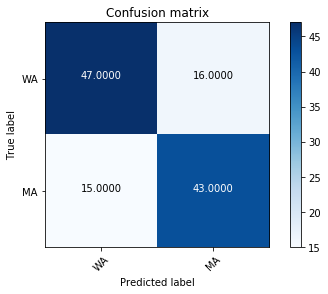
\includegraphics{Figure/SVMCM.png}}
\caption{Confusion Matrix of SVM} \label{fig:CMSVM}
\end{figure}


\begin{figure}
\centering
\scalebox{0.6}{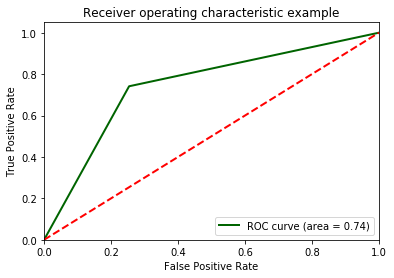
\includegraphics{Figure/SVMROC.png}}
\caption{ROC of SVM} \label{fig:ROCSVM}
\end{figure}


\begin{table}[h]
\center
\caption{Estimation result for SVM}
\scalebox{0.99}{
\begin{tabular}{|c|c|}
\hline
Results & Number\\\hline
Accuracy & 74\%\\\hline
Recall & 74\%\\\hline
Precision & 73\%\\\hline
\end{tabular}}
\label{tab:SVM}
\end{table}

Logistic Regression: Confusion matrix is in Figure \ref{fig:CMLR}, and ROC is in Figure \ref{fig:ROCLR}. The accuracy, recall and precision is in table \ref{tab:LR}.


\begin{figure}
\centering
\scalebox{0.6}{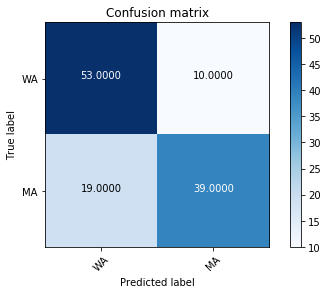
\includegraphics{Figure/LRCM.png}}
\caption{Confusion Matrix of Logistic Regression} \label{fig:CMLR}
\end{figure}


\begin{figure}
\centering
\scalebox{0.6}{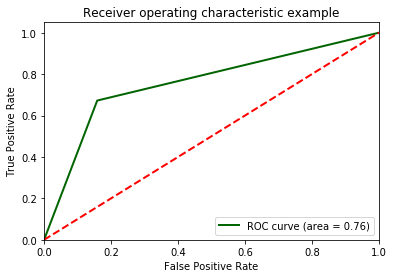
\includegraphics{Figure/LRROC.png}}
\caption{ROC of Logistic Regression} \label{fig:ROCLR}
\end{figure}


\begin{table}[h]
\center
\caption{Estimation result for Logistic Regression}
\scalebox{0.99}{
\begin{tabular}{|c|c|}
\hline
Results & Number\\\hline
Accuracy & 76\%\\\hline
Recall & 67\%\\\hline
Precision & 80\%\\\hline
\end{tabular}}
\label{tab:LR}
\end{table}

Naive Bayes Classifier: Confusion matrix is in Figure \ref{fig:CMNBC}, and ROC is in Figure \ref{fig:ROCNBC}. The accuracy, recall and precision is in table \ref{tab:NBC}.


\begin{figure}
\centering
\scalebox{0.6}{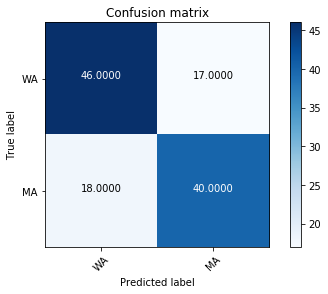
\includegraphics{Figure/NBCCM.png}}
\caption{Confusion Matrix of Naive Bayes Classifier} \label{fig:CMNBC}
\end{figure}


\begin{figure}
\centering
\scalebox{0.6}{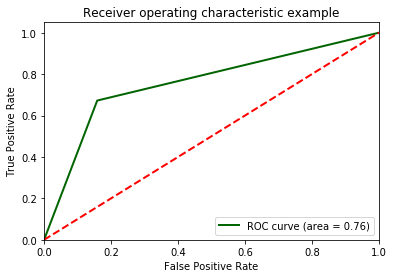
\includegraphics{Figure/LRROC.png}}
\caption{ROC of Naive Bayes Classifier} \label{fig:ROCNBC}
\end{figure}


\begin{table}[h]
\center
\caption{Estimation result for Naive Bayes Classifier}
\scalebox{0.99}{
\begin{tabular}{|c|c|}
\hline
Results & Number\\\hline
Accuracy & 71\%\\\hline
Recall & 69\%\\\hline
Precision & 70\%\\\hline
\end{tabular}}
\label{tab:NBC}
\end{table}


\newpage

\section{Define Own Project}
\textbf{Question 16:}
Prediction Based on Sentiment Analysis

(1)Show the value of sentiment analysis for each tweet in each time periods in ‘#gopatriots’ and ‘#gohawks’ in a figure.

For '#gopatruits', the plots of data point number vs value of setiments for 9 different day time are in Figure \ref{fig:q161},\ref{fig:q162},\ref{fig:q163},\ref{fig:q164},\ref{fig:q165},\ref{fig:q166},\ref{fig:q167},\ref{fig:q168}, and \ref{fig:q169}.


\begin{figure}
\centering
\scalebox{0.6}{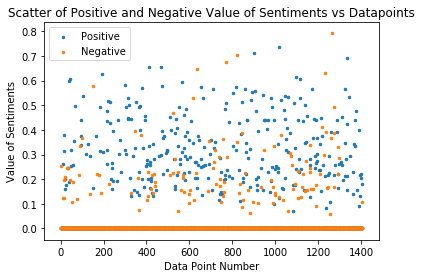
\includegraphics{Figure/q161.png}}
\caption{Data point number 1} \label{fig:q161}
\end{figure}

\begin{figure}
\centering
\scalebox{0.6}{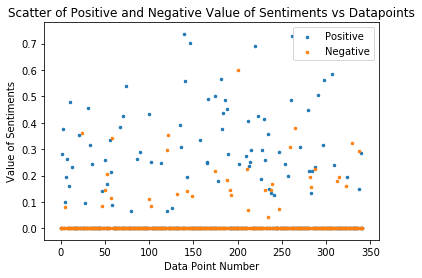
\includegraphics{Figure/q162.png}}
\caption{Data point number 2} \label{fig:q162}
\end{figure}

\begin{figure}
\centering
\scalebox{0.6}{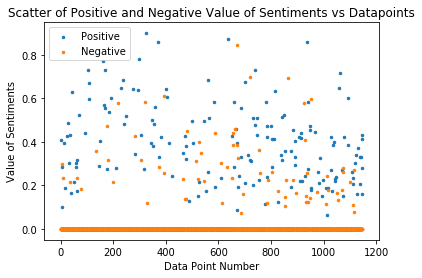
\includegraphics{Figure/q163.png}}
\caption{Data point number 3} \label{fig:q163}
\end{figure}

\begin{figure}
\centering
\scalebox{0.6}{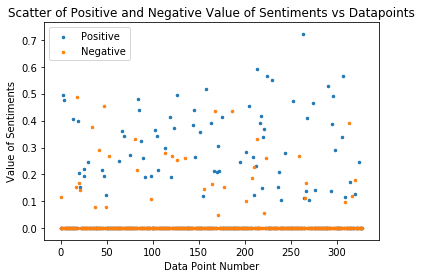
\includegraphics{Figure/q164.png}}
\caption{Data point number 4} \label{fig:q164}
\end{figure}

\begin{figure}
\centering
\scalebox{0.6}{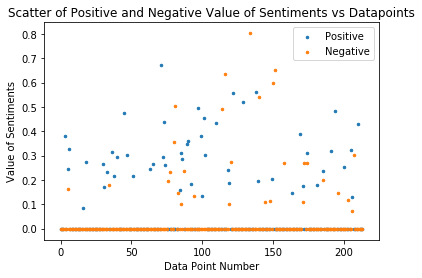
\includegraphics{Figure/q165.png}}
\caption{Data point number 5} \label{fig:q165}
\end{figure}

\begin{figure}
\centering
\scalebox{0.6}{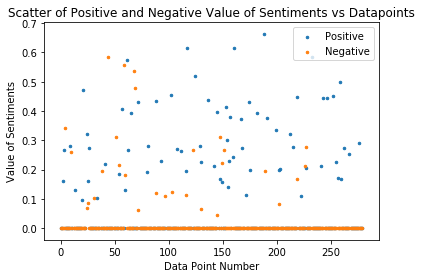
\includegraphics{Figure/q166.png}}
\caption{Data point number 6} \label{fig:q166}
\end{figure}

\begin{figure}
\centering
\scalebox{0.6}{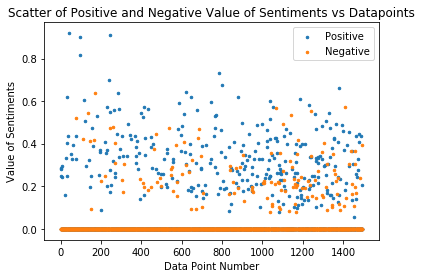
\includegraphics{Figure/q167.png}}
\caption{Data point number 7} \label{fig:q167}
\end{figure}

\begin{figure}
\centering
\scalebox{0.6}{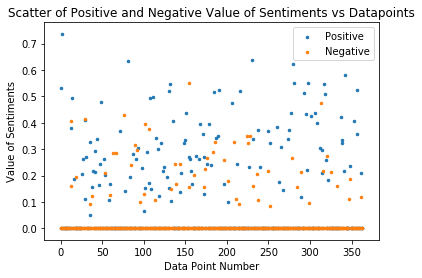
\includegraphics{Figure/q168.png}}
\caption{Data point number 8} \label{fig:q168}
\end{figure}

\begin{figure}
\centering
\scalebox{0.6}{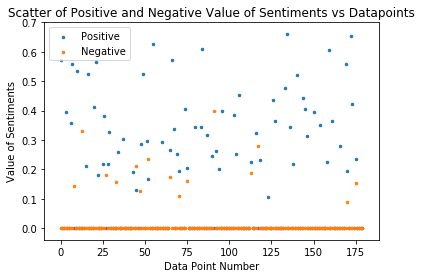
\includegraphics{Figure/q169.png}}
\caption{Data point number 9} \label{fig:q169}
\end{figure}


For '#gohawks', the plots of data point number vs value of setiments for 9 different day time are in Figure \ref{fig:q1611},\ref{fig:q1621},\ref{fig:q1631},\ref{fig:q1641},\ref{fig:q1651},\ref{fig:q1661},\ref{fig:q1671},\ref{fig:q1681}, and \ref{fig:q1691}.\\


\begin{figure}
\centering
\scalebox{0.6}{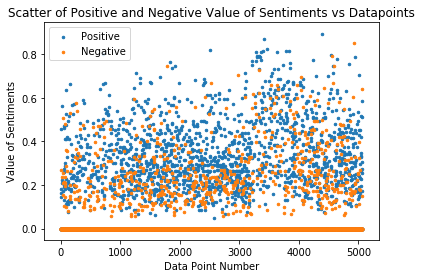
\includegraphics{Figure/q1611.png}}
\caption{Data point number 1} \label{fig:q1611}
\end{figure}

\begin{figure}
\centering
\scalebox{0.6}{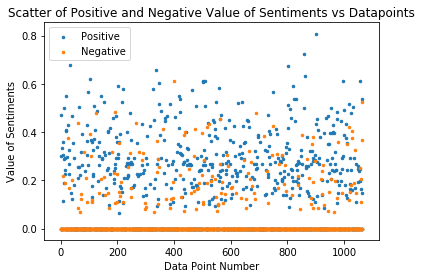
\includegraphics{Figure/q1621.png}}
\caption{Data point number 2} \label{fig:q1621}
\end{figure}

\begin{figure}
\centering
\scalebox{0.6}{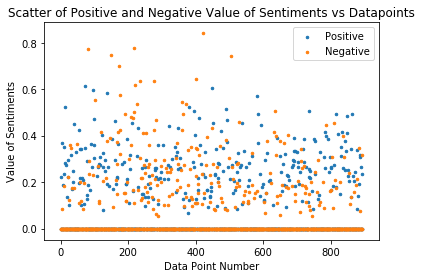
\includegraphics{Figure/q1631.png}}
\caption{Data point number 3} \label{fig:q1631}
\end{figure}

\begin{figure}
\centering
\scalebox{0.6}{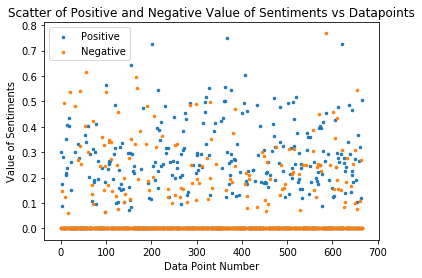
\includegraphics{Figure/q1641.png}}
\caption{Data point number 4} \label{fig:q1641}
\end{figure}

\begin{figure}
\centering
\scalebox{0.6}{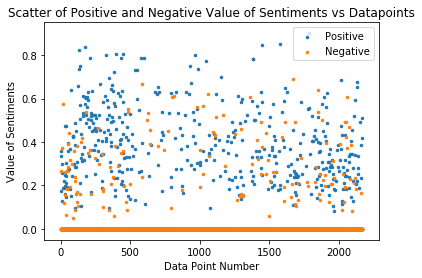
\includegraphics{Figure/q1651.png}}
\caption{Data point number 5} \label{fig:q1651}
\end{figure}

\begin{figure}
\centering
\scalebox{0.6}{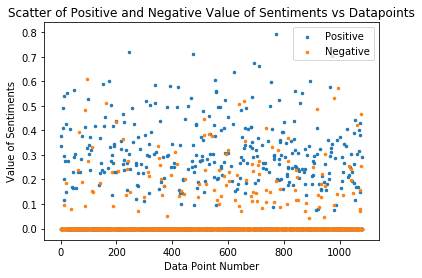
\includegraphics{Figure/q1661.png}}
\caption{Data point number 6} \label{fig:q1661}
\end{figure}

\begin{figure}
\centering
\scalebox{0.6}{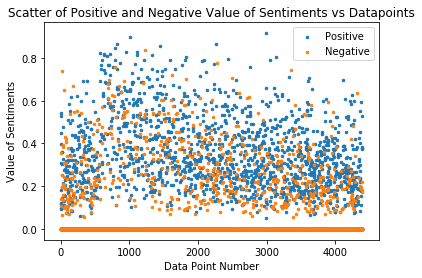
\includegraphics{Figure/q1671.png}}
\caption{Data point number 7} \label{fig:q1671}
\end{figure}

\begin{figure}
\centering
\scalebox{0.6}{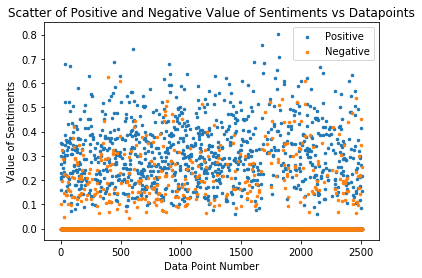
\includegraphics{Figure/q1681.png}}
\caption{Data point number 8} \label{fig:q1681}
\end{figure}

\begin{figure}
\centering
\scalebox{0.6}{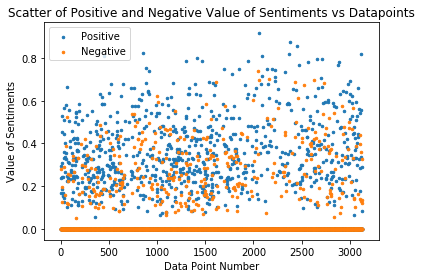
\includegraphics{Figure/q1691.png}}
\caption{Data point number 9} \label{fig:q1691}
\end{figure}



(2)Show the number of positive and negative tweets in each time periods as a plot, and also show the ratio of positive and negative accordingly in a plot.

For 'gopatruits', the number of tweets in positive and negative sentiments vs time period is in Figure \ref{fig:q16_21}. The rate of positive and negative tweets vs time period is in Figure \ref{fig:q16_22}.

For 'gohawks', the number of tweets in positive and negative sentiments vs time period is in Figure \ref{fig:q16_23}. The rate of positive and negative tweets vs time period is in Figure \ref{fig:q16_24}.\\

\begin{figure}
\centering
\scalebox{0.6}{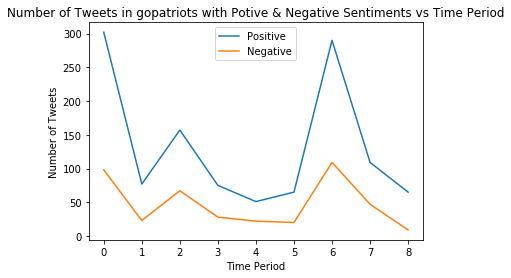
\includegraphics{Figure/q16_21.png}}
\caption{the number of tweets in positive and negative sentiments vs time period for 'gopatruits'} \label{fig:q16_21}
\end{figure}

\begin{figure}
\centering
\scalebox{0.6}{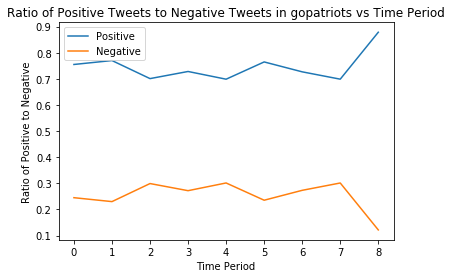
\includegraphics{Figure/q16_22.png}}
\caption{The rate of positive and negative tweets vs time period for 'gopatruits'} \label{fig:q16_22}
\end{figure}

\begin{figure}
\centering
\scalebox{0.6}{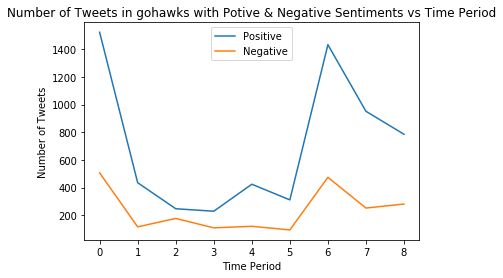
\includegraphics{Figure/q16_23.png}}
\caption{the number of tweets in positive and negative sentiments vs time period for 'gohawks'} \label{fig:q16_23}
\end{figure}

\begin{figure}
\centering
\scalebox{0.6}{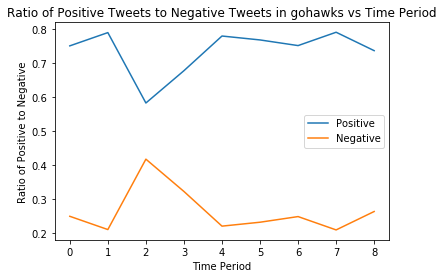
\includegraphics{Figure/q16_24.png}}
\caption{The rate of positive and negative tweets vs time period for 'gohawks'} \label{fig:q16_24}
\end{figure}

(3)Based on the statistics for the sentiment analysis of tweets for two opponent teams above and the time of goal in this game, build a linear regression model based on tweets to predict which team will win finally.

After training a linear regression model, the final accuracy is 44.4\%. The plot of predict value vs true value for hawks is in Figure \ref{fig:q16res}.

\begin{figure}
\centering
\scalebox{0.6}{\includegraphics{Figure/q16result.png}}
\caption{predict value vs true value for hawks} \label{fig:q16res}
\end{figure}


\end{document}
